\chapter{Experimental Assessment of IaaS Clouds}\label{cap:evaliaas}

\noindent In this chapter we will be reviewing the most used frameworks to drive IaaS Clouds. An initial selection will be made and it will be progressively shrunk following certain criteria like maturity, ease of use or documentation quality, until one remains. A deep study will be carried out on that prevailing one.

\section{Metodolog\'ia de evaluaci\'on}\label{sec:evaluacion}

\noindent A thorough evaluation of the capabilities of the different frameworks is not possible unless an actual deployment is carried through. The virtual infrastructure that is generated when a cloud has finished installing, no matter how small the deployment, is large and complex. Besides, trying to \emph{emulate} the real hardware that will support the cloud is meager at times, e.g. if full hardware virtualization were used, the hypervisor would have to be allowed direct access to the CPU. \emph{Nested Hardware Virtualization} --- the capacity for a CPU to export its native virtualization capabilities to a guest running atop a host node, or the ability to use full hardware virtualization \emph{inside} a virtual machine ---, does not currently enjoy widespread adoption as it requires implementation efforts from both CPU designers and virtualization software developers. This means that it will not be possible for us to fully appraise the myriad IaaS Cloud solutions by creating a virtual cluster over which to deploy our clouds, and make performance measures.

To diagnose the superiority of one of them over the rest, a scaled down setup will be completed to evaluate the proficiency in maintaining the IaaS service running in spite of the reduced infrastructure. Quality and transparency in the documentation, as well as community support and engagement will also be born in mind.

The testing environment follows the organization shown in figure \ref{fig:espacioprueba}.

\begin{figure}[tbp]
\begin{center}
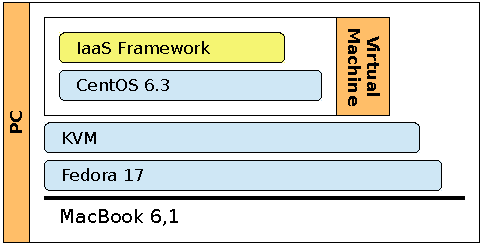
\includegraphics[width=0.55\textwidth]{imagenes/007.pdf}
 \caption{General testing space}
\label{fig:espacioprueba}
\end{center}
\end{figure}

\section{Evaluated Frameworks}\label{sec:frameworksevaluados}

\noindent The frameworks are:
\begin{itemize}
 \item CloudStack %3.0.2
 \item Eucalyptus %3.1.1
 \item OpenNebula %3.8.1
 \item OpenStack
\end{itemize}

From an exclusively functional vantage point, the four of them cover clearly the requirements imposed with the project, which, in short, it would be the faculty to run and manage the lifecycle of an indeterminate number of custom VMs, tailored for MapReduce executions, through an API that would allow for the definition of a simple job control interface.

\emph{Eucalyptus} and \emph{OpenStack} take a more modular approach to the solution, unveiling smaller functional parts, while at the same time decoupling those modules. With a module set in this fashion, installations become more flexible and tougher on par. However, to contain the operative effort, OpenStack ships with a series of scripts that help managing its deployments. Regarding their system requirements, they all support installations in modern Linux distributions with KVM or Xen as hypervisors. When dealing with a real deployment, the framework of choice will likely depend more on the existing platform than on particular limitations that any cloud may have.

As a side note, it is remarkable the lack of interoperability among them. All of them try to adhere to the AWS API in different degree --- some of them partially support it, others use \emph{adaptors} to it. OpenNebula, OpenStack and Eucalyptus have demonstrated to be carrying on coding efforts to fully support the OGF's standard: OCCI.

%\subsection{Eucalyptus}\label{subsec:eucaliptus}

Eucalyptus, in spite of being the first to fully cover the AWS API, which is merely anecdotical nowadays, has two obstacles that hinder its evaluation. First, it is not fully open sourced:\texttt{VMware Broker} which brings the opportunity to use virtualized infrastructure based on  VMware technology, is only available to paid subscribers. And second, it is impossible to setup Eucalyptus within a VM to test start-up time or installation complexity, for example, as it explains its installation guide \cite{eucainstall}. Both limitations make Eucalyptus back out from the evaluation list. The rest have been compared after their set up and configuration.

\subsection{CloudStack}\label{subsec:cloudstack}

\noindent CloudStack installation guide (\cite{cloudstackquickinstall}) describes the series of steps that a systems engineer should follow in order to complete a minimum CloudStack deployment. It clearly determines that Cloud Nodes' CPUs have to support virtualization extensions for CloudStack to start Xen or KVM-based VMs. Which happens to be a similar limitation to Eucalyptus'. However, the fact that CloudStack would become part of \emph{The Apache Software Foundation} from version 4 onward (\cite{cloudstackstrategy}), and the reality of a Citrix technical article opening the door to CloudStack deployments over Cloud Nodes lacking virtualization extensions (\cite{apachecloudstack4}), made us arrange the layout shown in figure \ref{fig:cloudstack}.

\begin{figure}[tbp]
\begin{center}
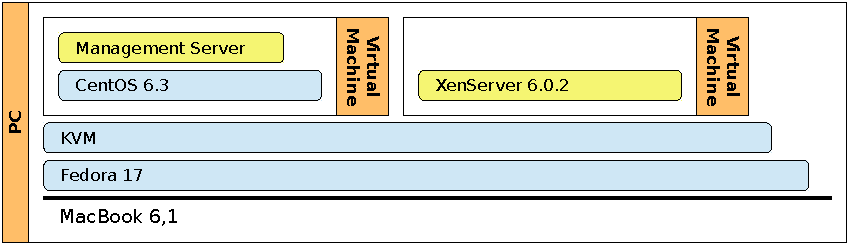
\includegraphics[width=0.99\textwidth]{imagenes/008.pdf}
 \caption{CloudStack 3.0.2 with XenServer hypervisor}
\label{fig:cloudstack}
\end{center}
\end{figure}

Following the advanced and quick installation guides --- \cite{cloudstackquickinstall} and \cite{cloudstackadvinstall} --- the process may be summarized in the steps bellow:

\begin{itemize}
 \item Two VMs were created to contain CloudStack \emph{Management Server} (\emph{MS}) and XenServer hypervisor: 1 GB of RAM for the MS, 3 GB of RAM for Xen, 20 GB HDD, \emph{ACPI} and \emph{APIC} for both.
 \item For the MS:
  \begin{itemize}
   \item \emph{CentOS 6.3} was downloaded, installed and \texttt{yum-updated}.
   \item The VM was named \emph{cloudstack}.
   \item Likewise, a user named \emph{cloudstack} was registered and added to the \emph{sudoers} list.
   \item The quick installation guide was followed to conclude the process.
  \end{itemize}
 \item For Xen:
  \begin{itemize}
   \item XenServer 6.0.2 was downloaded from Citrix web site.
   \item The notes contained in the quick installation guide and in the XenServer configuration manual \cite{xenserinstall} were followed to perform the configuration.
  \end{itemize}
  \item Additionally:
   \begin{itemize}
    \item Before specifying the execution environment, defining the cluster, primary and secondary storage, etc. a global flag had to be set to permit nodes with no virtualization extensions \cite{cloudstacknohvm}.
    \item Once the configured infrastructure was online:
     \begin{itemize}
      \item The CentOS 6.3 image was uploaded to the MS.
      \item A \texttt{SimpleHTTPServer} --- a Python micro HTTP server --- was started on port \emph{443} in the MS.
      \item A rule was added in \texttt{iptables} to let traffic through on port \emph{443} in the MS.
      \item The image was loaded to the cloud from the web interface.
     \end{itemize}
   \end{itemize}
\end{itemize}

\subsection{OpenNebula}\label{subsec:opennebula}

\noindent If balanced against the installation procedure just described, the effort for setting up OpenNebula 3.8 is lighter. The process that has been followed to configure the OpenNebula deployment contained in figure \ref{fig:opennebula} stems directly from \cite{centosonquickstart}, the official installation guide. The subsequent steps serve as summary to the process.

\begin{figure}[tbp]
\begin{center}
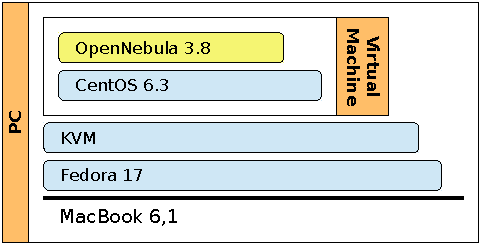
\includegraphics[width=0.55\textwidth]{imagenes/009.pdf}
 \caption{OpenNebula 3.8 with KVM}
\label{fig:opennebula}
\end{center}
\end{figure}

\begin{itemize}
 \item Se cre\'o una m\'aquina virtual soporte para todo el cloud OpenNebula: 1 GB RAM, 8 GB HDD, ACPI y APIC.
 \item Se descarg\'o, instal\'o y actualiz\'o CentOS 6.3.
 \item Se nombr\'o \emph{opennebula} a la m�quina virtual.
 \item Igualmente nombrado, se dio de alta un nuevo usuario, \emph{opennebula}, y se agreg\'o a la lista de \emph{sudoers}.
 \item Se detuvo \texttt{SELinux}.
 \item Se sigui\'o la gu\'ia contenida en \cite{centosonquickstart} para concluir el proceso, al que hubo que integrar las siguientes cuestiones para probar el framework:
  \begin{itemize}
   \item Por defecto, el servicio que brinda la interfaz web de OpenNebula (\texttt{sunstone}) se engancha en \emph{lo}. Para que pudiera ser accedido desde fuera del servidor, fuera de la m\'aquina virtual en este caso, fue necesario precisar que sunstone habr\'ia de escuchar en \emph{eth0}, modificando, para este fin, la configuraci\'on correspondiente en \texttt{/etc/one}. Lo mismo aconteci\'o con \texttt{occi}, el servicio REST de control del cloud.
   \item Adicionalmente, se agreg\'o a iptables la regla para no filtrar el tr\'afico en el puerto \texttt{9869}, el de sunstone inicialmente.
  \end{itemize}
\end{itemize}


\subsection{OpenStack}\label{subsec:openstack}
\noindent El caso de OpenStack es llamativo por varias razones. Representa la convergencia entre dos necesidades diferentes: la puramente computacional de la NASA y la orientada al almacenamiento de Rackspace. Complementariamente, tanto Red Hat como Canonical han sumado su aporte bajo la forma de scripts de instalaci\'on y control en el caso de Red Hat, y escribiendo utilidades de despliegue autom\'atico, como \texttt{juju}, en el caso de Canonical.\newline

Como en el caso de OpenNebula, se configur\'o un entorno de ejecuci\'on contenido en una sola m\'aquina virtual. En este caso se eligi\'o a Fedora frente a CentOS y Ubuntu por el soporte comunitario en forma de extensa gu\'ia de instalaci\'on r\'apida \cite{quickstartfedoraos} y por la existencia de herramientas que ace\-le\-ra\-r\'ian sustancialmente el procedimiento. La gu\'ia de instalaci\'on y despligue oficial de OpenStack Folsom \cite{installdeployosfolsom}, est\'a escrita centr\'andose excesivamente en Ubuntu, lo que se tradujo en comandos no aplicables en Fedora. Como \'ultimo comentario previo a la descripci\'on de la puesta en marcha, decir que se probaron dos versiones de OpenStack: \emph{Essex} y \emph{Folsom}. La raz\'on radica en el hecho de que, a pesar de ser Essex la soportada oficialmente por la distribuci\'on (Fedora 17), desde la gu\'ia r\'apida mencionada anteriormente \cite{quickstartfedoraos} se recomendaba usar la \'ultima versi�n de OpenStack disponible ---Folsom a diciembre de 2012---, habilitando un re\-po\-si\-to\-rio de avance a tal fin.\newline

El grado de madurez observado de Folsom frente a Essex es sustancialmente llamativo en la interfaz web: lo que parec\'ia una primera aproximaci\'on para formular comandos de administraci\'on del cloud, evolucion\'o hacia una interfaz mucho m\'as cohesionada con el comportamiento real. El ejemplo si\-guien\-te pone de manifiesto esta idea: en el momento de lanzar instancias para probar el correcto funcionamiento del cloud, se observ\'o que, en caso de existir alg\'un problema de configuraci\'on en el subsistema de red que impidiese que las instancias obtuviesen direcciones IP, \'estas permanec\'ian en un estado que hac\'ia imposible su eliminaci\'on desde la interfaz web. Fue necesario recurrir a la edici\'on de la base de datos y la estructura de ficheros del controlador del cloud, con algunos resultados nefastos como la p\'erdida de informaci\'on de uso de las instancias, para restablecer la coherencia en Essex. El mismo problema se solventa directamente en Folsom (tanto desde la interfaz web como desde la l\'inea de comandos).\newline

Siguiendo el \'indice siguiente se dispuso un entorno de ejecuci\'on id\'entico para sendas versiones (ver figura \ref{fig:openstack}).

\begin{figure}[tbp]
\begin{center}
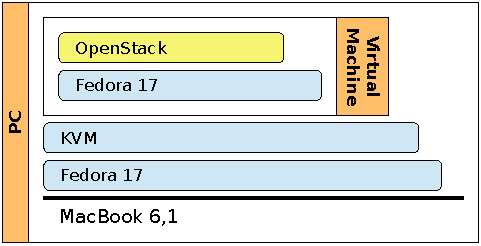
\includegraphics[width=0.55\textwidth]{imagenes/010.pdf}
 \caption{OpenStack en despligue virtual}
\label{fig:openstack}
\end{center}
\end{figure}

\begin{itemize}
 \item Se cre\'o una m\'aquina virtual para todo el cloud OpenStack: 1 GB RAM, 10 GB HDD, APIC y ACPI.
 \item Se descarg\'o, instal\'o y actualiz\'o Fedora 17.
 \item Se nombr\'o \emph{openstack} a la m\'aquina virtual.
 \item Igualmente nombrado, se dio de alta un nuevo usuario, \emph{openstack}, y se agreg\'o a la lista de \emph{sudoers}.
 \item Se instal\'o el paquete \texttt{acpid} para poder controlar los aspectos de energ\'ia desde el manejador de cloud.
 \item Se detuvo SELinux.
 \item Se orden\'o una copia en profundidad de la m\'aquina virtual ---tanto configuraci\'on de la m\'aquina como HDD--- para probar Essex y Folsom, y se renombraron convenientemente.
 \item Se siguieron tanto la gu\'ia de instalaci\'on r\'apida extraoficial \cite{quickstartfedoraos}, como la gu\'ia oficial de despliegue \cite{installdeployosfolsom}, dejando de lado la con\-fi\-gu\-ra\-ci\'on de \texttt{Swift}, para concluir el procedimiento.
 \item A mayores, se crearon sendos discos virtuales de 4 GB para albergar los vol\'umenes del almacenamiento de bloque gestionados por \texttt{Compute}, para Essex, y \texttt{Cinder} para Folsom.
\end{itemize}
 

\section{Conclusiones}\label{sec:conclusiones}
\noindent Presentamos, seguidamente, los resultados de la comparaci\'on de los frameworks de IaaS, atendiendo a las cuestiones resaltadas en la metodolog\'ia.
 
\begin{description}
 \item[Instalaci\'on:] Sin lugar a dudas OpenNebula se lleva la palma. La gu\'ia de instalaci�n es, con mucho, la m\'as corta y ligera de seguir. Acarrea, no obstante, el problema de tener un desconocimiento mayor de lo que est\'a sucediendo bajo la superficie, que dificultar\'a la resoluci\'on de los problemas que pudieran aparecer, as� como el manejo general del cloud.
 \item[Configuraci\'on y manejo:] El aprovisionamiento de nueva infraestructura, es decir, la uni\'on de nuevos anfitriones al cloud, requiere, en todos los frameworks analizados, la instalaci\'on en cada anfitri\'on del hipervisor que se pretenda utilizar. CloudStack y OpenNebula ofrecen una gesti\'on mucho m\'as transparente que OpenStack, siendo necesario ma\-yor esfuerzo de instalaci\'on y configuraci\'on. En este \'ultimo adem\'as, la interfaz web no deja forma alguna de conocer el tama\~no del cl\'uster real sobre el que corre el cloud ni, l\'ogicamente, el grado de utilizaci\'on de la infraestructura. Entre CloudStack y OpenNebula la diferencia es inexistente en cuanto a la funcionalidad expuesta a trav\'es de sus webs. CloudStack expone los servicios de todo el cloud como una jerarqu\'ia; OpenNebula como una tabla.
 \item[Hipervisor:] En cuanto a hipervisores soportados se refiere, OpenStack aventaja claramente a CloudStack y OpenNebula. Sin embargo, se podr\'ia afirmar que este hecho es pr\'acticamente anecd\'otico porque los tres soportan los m\'as conocidos ---KVM, Xen, variantes de Xen y variantes de VMWare--- que son los utilizados en casi todos los despliegues reales.
 \item[Almacenamiento:] Los tres soportan una m\'as que surtida variedad de controladores de \emph{backend} de datos. Pero, en este caso, es importante subrayar el esfuerzo de OpenStack por implementar la funcionalidad ofrecida por Amazon S3 ---almacenamiento en cloud r\'apido y seguro. Swift es el componente de OpenStack que otorga almacenamiento tolerante a fallos y de alta disponibilidad a los despliegues, sustent\'andose para lograrlo en la replicaci\'on y el balanceo de carga, entre otros. La gu\'ia avanzada de instalaci\'on de CloudStack \cite{cloudstackadvinstall}, muestra una primera aproximaci\'on para la configuraci\'on de Swift como almacenamiento secundario del cloud. De ah\'i se puede deducir en cierto grado la importancia y madurez de Swift como m\'odulo de OpenStack.
 \item[Documentaci\'on:] Ninguno de los tres puede presumir de manuales de instalaci\'on oficiales correctos al 100\%. Adem\'as, como se da la circunstancia de que cada framework ha ido madurando con grados de exposici\'on diferentes a las diversas distribuciones Linux, la cobertura que ofrecen para cada sistema operativo es muy heterog\'enea; hasta el punto de confundir, en alg\'un caso, los nombres de los m\'odulos cuyas funciones hay que invocar. Por ejemplo, ambos manuales de instalaci\'on de CloudStack ---r\'apida \cite{cloudstackadvinstall} y avanzada \cite{cloudstackquickinstall}--- se siguen m\'as correctamente usando CentOS como sistema operativo de base y XenServer como hipervisor. OpenStack dispone oficialmente de manuales de ins\-ta\-la\-ci\'on que soportan tanto derivados de Red Hat ---Fedora, CentOS, el propio Red Hat Enterprise Linux, etc.--- como de Debian ---Ubuntu, Debian, etc.--- sin embargo, al realizar el despliegue sobre Fedora se observ\'o que el nombre de los servicios documentados no se correspond\'ia con el nombre real; en Ubuntu no sucede tal cosa. De todas formas, las incorrecciones son nimias y la extensi\'on de la documentaci\'on es m\'as que suficiente para despliegues en producci\'on.
 \item[Comunidad:] A pesar de que pueda resultar algo secundario, la calidad del soporte comunitario es vital para el desarrollo y soporte de los frameworks. Todos ellos est\'an compuestos por m\'odulos escritos en c\'odigo abierto y libre en su mayor parte, de forma que, cuanto mayor sea el bullicio recogido en foros de desarrollo, mayor ser\'a tambi\'en el aporte recibido; y as\'i, el grado de madurez operativo, funcional y documental ser\'a mayor. A pesar de que no pueda darse un claro vencedor en este apartado, debido al car\'acter difuso de la magnitud \emph{soporte comunitario}, s\'i es interesante destacar el importante apoyo a OpenStack de Canonical y Red Hat: no hay conferencia o charla t\'ecnica general de uno u otro donde no hagan referencia a OpenStack.
\end{description}

\subsection{OpenStack Folsom}\label{subsec:openstackfolsom}
\noindent Finalmente, el framework para cloud IaaS elegido es OpenStack Folsom. Las gu\'ias de instalaci\'on mencionadas, el soporte comunitario, el empuje por parte de dos pesos pesados del software, los despliegues reales de HP, Dell, Intel, Rackspace, etc., la modularidad de configuraci\'on, la completitud de implementaci\'on (soporte de los APIs OCCI, S3, EC2 y definici\'on de un servicio de almacenamiento en cloud como Swift) y el soporte oficial de despliegue de prueba sobre m\'aquinas virtuales ---usando emulaci\'on--- han desequilibrado la balanza a su favor.
